%%%%%%%%%%%%% ptdr definitions %%%%%%%%%%%%%%%%%%%%%
\input{ptdr-definitions}

\newcommand{\pp}{\ensuremath{\mathrm{pp}}}%
\newcommand{\Wo}{\ensuremath{\mathrm{W}}}%
\newcommand{\Zo}{\ensuremath{\mathrm{Z}}}%
\newcommand{\rts}{\ensuremath{\sqrt{s}}}%
\newcommand{\ra}{\ensuremath{\rightarrow}}%
\newcommand{\MN}{\ensuremath{\mu\nu}}%
\newcommand{\MW}{\ensuremath{\mathrm{m}_\Wo}}%
\newcommand{\MZ}{\ensuremath{\mathrm{m}_\Zo}}%
\newcommand{\MT}{\ensuremath{\mathrm{M}_T}}%

\newcommand{\Wmn}{\ensuremath{\Wo \ra \MN}}%
\newcommand{\Zmm}{\ensuremath{\Zo \ra \MM}}%
\newcommand{\Wtn}{\ensuremath{\Wo \ra \tau\nu}}%
\newcommand{\Ztt}{\ensuremath{\Zo \ra \tau\tau}}%
\newcommand{\ppZmm}{\pp \ra \Zo + X \ra \MM + X}%
\newcommand{\ppWmn}{\pp \ra \Wo + X \ra \MN + X}%

%%%%%%%%%%%%%%%  Title page %%%%%%%%%%%%%%%%%%%%%%%%
\cmsNoteHeader{XXX/YYY}
\title{Study of the Barrel RPC L1 Trigger efficiency \\
with a muon sample triggered by the DT system}
% Force line breaks with \\

%Author is always "The CMS Collaboration" for PAS, so author, etc will be ignored
\address[nap]{INFN and Universit{a'} di Napoli}
\address[bari]{INFN and Universita' di Bari}
\author[nap]{F.~Fabozzi}
\author[nap]{A.O.M.~Iorio}
\author[bari]{R.~Trendadue}

% please supply the date in yyyy/mm/dd format. Today has been
% redefined to do so, but it should be fixed as of the final release date.
%\date{\today}

% note that you cannot use \verb in the abstract text
\abstract{
    We present a study of the L1 trigger efficiency for RPCs in the
    Barrel of the CMS Muon System. The method exploits the independency of the
    DT and RPC trigger systems. Muon tracks in the event are 
    triggered and reconstructed using the DT system only, and for each of
    them we search for a compatible RPC L1 trigger object. 
    We discuss in detail the results obtained on a few good 
    runs taken from CRAFT08 and CRAFT09 datasets. The algorithm has been 
    released in the Prompt Analysis Framework of the RPC system for a fast
    off-line monitoring of the trigger performances.
}

% these need to be filled in by hand and should (MUST) match the info
% in the TeX equivalents less the TeX markup
%\hypersetup{%
%pdfauthor={Francesco Fabozzi},%
%pdftitle={Towards a measurement of W and Z cross sections into muons in pp collisions at rts=10 TeV},%
%pdfsubject={CMS},%
%pdfkeywords={CMS, physics, software, computing}}

\maketitle %maketitle comes after all the front information has been supplied

%%%%%%%%%%%%%%%%%%%%%%%%%%%%%%%%  Begin text %%%%%%%%%%%%%%%%%%%%%%%%%%%%%
\section{Introduction}
The CMS Muon System~\cite{ref:mutdr}\cite{ref:jinst} has 
been designed to provide excellent muon
identification, triggering and precise momentum reconstruction 
over the entire kinematic range foreseen at LHC. A crucial
feature of the system is the redundancy provided by the DT/RPC 
(CSC/RPC) independent sub-systems in the Barrel (Endcap) region.
In particular, the RPC system is able to provide 
a fast and higly segmented trigger [ref trig TDR], with a 
sharp \pt threshold, in the rapidity range $|\eta| < 1.6$.
The independence of the DT and RPC systems can be exploited
to develop a method for the measurement of the Barrel RPC L1 
trigger efficiency, which can be extremely useful 
for a prompt monitoring of system performances.
In this note we discuss this method and present results
obtained on CRAFT08 and CRAFT09 cosmic data samples.
The method can be also adapted to measure the 
trigger efficiency of the RPCs in the Endcap region.

\section{The Barrel RPC system}
In this section we briefly describe the layout of the
Barrel RPC system just to introduce some
naming conventions. Detailed descriptions
can be found in References \cite{ref:mutdr}
and \cite{ref:jinst}.

The Barrel Muon System is composed of 5 Wheels along 
the $z$ direction, named W-2, W-1, W0 (the central one), 
W+1, W+2. Each wheel is divided into twelve 
sectors (with approximately dodecagonal geometry in the 
$r$-$\phi$ view), from sector S0 to sector S12 
(see Fig.~\ref{fig:barrel_lay}).

\begin{figure}[hbtp]
  \begin{center}
    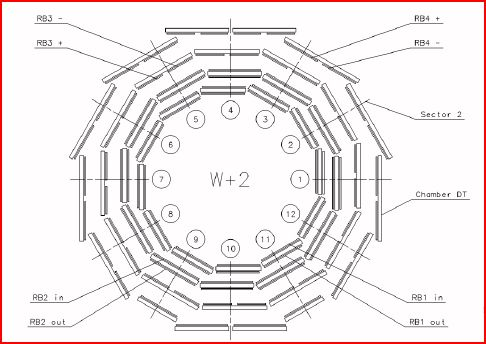
\includegraphics[width=0.8\textwidth]{barrel_layout}
    \hspace{1cm}
    \caption{Transverse view of the Barrel RPC system.}
    \label{fig:barrel_lay}
  \end{center}
\end{figure}

For each sector there are 4 DT stations, inserted in the 
iron gaps of the Barrel Yoke, from MB1 (the inner one)
to MB4 (the outer one). 

The RPC stations are mounted on one or both sides of the DT 
stations. Station MB1 is provided with RPC stations on 
bottom and top sides (RB1In and RB1Out stations), same 
for MB2 (RB2In and RB2Out stations). Stations MB3 and MB4
are provided with RPC stations on the bottom side only
(RB3 and RB4 stations). 
With this design, a total of six concentric RPC layers are 
available in the Barrel Muon System. The inner
layers can provide up to four coordinate measurements also for 
low momentum tracks crossing only MB1 and MB2 stations.

For each RPC station, pick-up strips running parallel to the 
beam axis provide coordinate measurement in the $r$-$\phi$ view,
thus allowing \pt measurement of the track. 
Segmentation in the $\eta$ view is obtained by sectioning
a plane of strips in two or three parts. 
The $\eta$ partitions are called {\em rolls}.
An RPC station can be segmented into two rolls (named Backward and 
Forward) or three rolls (named Backward, Middle, and Forward).

\section{The L1 trigger system for Barrel RPCs}
From the point of view of the L1 trigger~\cite{ref:trig_tdr}, 
the RPC system volume is logically partitioned into 
sections. L1 trigger objects are searched 
for independently in each section.
Sections in the $\eta$ view will be referred as {\em towers},
and for each tower the partitions in  
in the $r$-$\phi$ view will be referred as {\em cones}.

\subsection{Trigger towers}
The definition of the $\eta$ boundaries 
of towers (see Fig.~\ref{fig:eta_towers}) is based on a set 
of reference stations.

\begin{figure}[hbtp]
  \begin{center}
    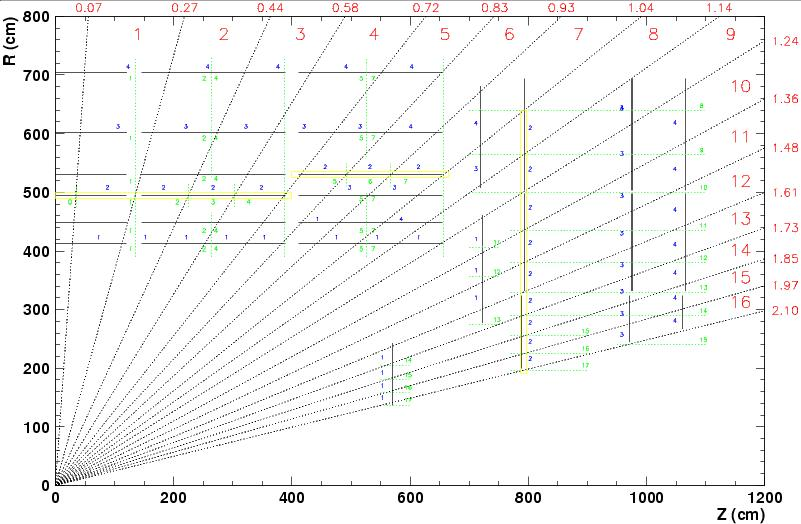
\includegraphics[width=0.8\textwidth]{eta_towers}
    \hspace{1cm}
    \caption{Trigger eta towers.}
    \label{fig:eta_towers}
  \end{center}
\end{figure}

In the Barrel, the reference stations are:
station RB2In for W+1, W0, and W-1, 
and station RB2Out for W-2 and W+2. 
Each tower must contain only one entire roll 
of a reference station. On the 
other hand, a roll of a non-reference station
can belong to adjacent towers, thus in this case 
the association of roll to towers is not univocally defined.
A total of 5+5+1 towers are entirely contained in the Barrel.

\subsection{Trigger cones}
On the reference stations, the strips are grouped in
non-overlapping sets of 8 adjacent strips called {\em segments}.
Each segment subtends a $\phi$ angle of $2.5^\circ$, for a total 
of 144 segments (12 segments for each sector).
Each cone must contain only one segment of a reference 
station.
On the other hand, in non-reference stations a larger number
of strips is grouped into a segment with overlaps 
between adjacent segments, making the association of a strip 
to a segment not univocally defined. Thus, the cones appear more 
like hourglass shaped partions.

\subsection{The L1 PACT logic}
The PAttern COmparator Trigger (PACT) logic 
collects RPC hits from all stations and searches for
spatial and time coincidences independently
in each cone. The $\eta$ and $\phi$ coordinate of the trigger
objects are assigned on the reference station.
By comparison with predefinite patterns of hits, 
also a \pt value is assigned to the candidate trigger 
object. Due to the overlap of adjacent cones, 
{\em ghost} trigger objects can appear. For this reason, 
the trigger objects found in a certain $\eta$ tower 
are processed by a proper ghost identification and removal logic,
and the remaining ones are sorted according to quality criteria.

Ghosts can also appear in adjacent towers due to the 
sharing of the rolls in non-reference stations.
For this reason, trigger candidates from all the towers are 
processed for ghosts removal, sorted according to 
quality criteria, and the 4 highest \pt muons
from the Barrel and the 4 highest \pt muons from the 
Endcap are finally sent to the Global Muon Trigger.

\subsection{Cosmic patterns in PACT}
In order to increase the trigger efficiency for 
cosmic muons, which are not constrained
to come from the interaction vertex, 
a looser pattern definition has been 
adopted with respect to collision runs.
A cosmic pattern is defined as a 
time coincidence of hits on at least
3 different RPC stations in a cone (3/6 majority).
No different patterns as a function 
of \pt are defined, thus the system is
not able to assign a \pt value 
to the track.

\section{Analysis method}
We start from a sample of reconstructed tracks 
in the Muon System which are matched to a DT 
trigger object, in order to remove fakes. If 
the number of tracks in the sample is
$N_{match}^{DT}$, and under the assumption
that RPC and DT triggers are uncorrelated,
the RPC trigger efficiency 
$\epsilon_{L1}^{RPC}$ is given by the fraction 
of tracks in the sample that are matched also 
to an RPC trigger object:
\begin{equation}
\epsilon_{L1}^{RPC} = N_{match}^{RPC\&DT}/N_{match}^{DT} \,\,\,.
\end{equation}

\subsection{Tracks selection}
For the analysis we use a collection of CosmicMuons.
CosmicMuons are made of tracks reconstructed in the
Muon System only.
The two legs of a muon which traverses
the Tracker System are reconstructed as two separate 
CosmicMuon tracks.
Kinematic parameters of a CosmicMuon track are given 
at its {\em innermost position}. 
For tracks in the top part of the detector
the innermost position is located on the outer stations
(because the track is going from top to bottom),
while for tracks in the bottom part it is located 
in the inner stations.
In order to prevent an eventual bias due to tracks 
that would not have been reconstructed without
RPC hits, we re-run the reconstruction using DT only.

We select cosmic tracks pointing to the $p$-$p$ interaction
region by requiring... 
The above cuts are applied at skim level.
(definition of TrackerPointing skim).

In addition, we apply the following 
cuts:
\begin{itemize}
\item
$\pt$ at the innermost point $ > 5\GeVc$;
\item
$N_{hits}$ in the DT $ > 20 $;
\item
$\chi^2$ of the track fit $ < 20 $.
\end{itemize}
The \pt cut removes tracks which are
looping in the transverse plane due 
to the magnetic bending (???).
The other two cuts ensure good quality
of the DT reconstruction and 
prevent an eventual bias due to 
tracks that would not have been triggered 
without RPC hits.
Figure xxx shows the distributions
of these variables for typical pointing
CosmicMuon tracks.

\subsection{Track matching with trigger objects}
The parameters of a reconstructed track are
measured at the innermost position, while the
parameters of the trigger objects are defined
at the reference station (which is the second station 
also for DT trigger).
Thus we propagate the track to the DT reference layer using 
{\em XXX}, an accurate propagation method through the CMS detector
geometry which takes into account the magnetic field, the 
energy loss in the detector material (and 
the multiple scattering???).
The distributions of $\eta$ and $\phi$ at the reference 
station for the tracks are shown in Fig.xxx. 
The track-trigger matching is performed in the $\phi$ coordinate 
only, which is the most accurate coordinate measured by both 
DT and RPC trigger systems. The $\phi$ distributions for DT and
RPC triggers objects are shown in Fig.xxx .


We first match the track to a DT trigger.
The matching requirement is $|\Delta\phi_{t-DT}| < 30^\circ$,
where $\Delta\phi_{t-DT}$ is the difference 
between the $\phi$ of the track at the reference station and 
the $\phi$ of the DT trigger. This loose requirement 
provides a high matching efficiency.

If we find a match with a DT trigger, then we proceed
for matching to an RPC trigger. 
Figure xxx shows the overall $\Delta\phi_{t-RPC}$ as measured 
using both cosmic patterns and collision patterns (the
last one obtained by running the trigger emulator).
The matching requirement is $|\Delta\phi_{t-RPC}| < 30^\circ$,
where $\Delta\phi_{t-RPC}$ is the difference 
between the $\phi$ of the track at the reference station 
and the $\phi$ of the RPC trigger.

\section{Data samples}
Only cosmic tracks which mimic muons from collisions
have been considered for this study. 
For this reason, we have analized runs taken from the 
following CRAFT08 and CRAFT09 datasets:
\begin{itemize}
\item
Commissioning08\/2213\_Tosca090322\_2pi\_scaled\_ReReco\_FromTrackerPointing-v1\/RAW-RECO
\item
Cosmics\/CRAFT09-PromptReco-v1\/RECO
\end{itemize}

The CRAFT08 dataset is a TrackerPointing skim, that is 
only cosmics pointing to the primary vertex 
region of CMS are selected. 
On the contrary, the CRAFT09 dataset is non-skimmed, 
since the pointing skim was not yet 
available. In this case we have filtered the 
events at the analysis level by applying the same
requirements used in the pointing skim.

Table~\ref{tab:runs} reports the run numbers analyzed and the relevant
conditions.
 \begin{table}[htb]
    \label{tab:runs}
    \begin{center}
      \begin{tabular}{|c|c|c|c|} \hline
Dataset & Run   & RPC HV & FEB threshold \\ \hline
CRAFT08 & 66783 & 9.2 kV & 220 mV \\ \hline
CRAFT09 & XXXXX & 9.4 kV & yyy \\ \hline
      \end{tabular}
      \caption{Analyzed runs from CRAFT08 
and CRAFT09 datasets. The HV value and FEB thresholds for
the RPC system are also reported.}
    \end{center}
  \end{table}


\section{RPC trigger efficiency in CRAFT08}
Here you have to present the results in CRAFT08.
I suggest:
\begin{itemize}
\item
2D efficiency plot; IMPORTANT: explain features of the plot 
\item
efficiency vs. eta towers
\item
define fiducial cuts and the reason for that
\item
plot integrated efficiency vs.pt using fiducial cuts
\item
quote the average eff.
\item
compare with tag and probe
\end{itemize}

\section{RPC trigger efficiency in CRAFT09}
Here you have to present the results
in CRAFT09.

\section{Discussion: CRAFT08 vs. CRAFT09}
Here you have to discuss the comparison
of results from 2008 vs 2009:
We should justify the change in the trigger efficiency.

\section{Conclusions}
Some conclusions: release the alghorithm in the prompt 
analysis system.
Perspective for analysis in collisions data samples.
Cross-check with MC truth efficiency by looking at 
a MC signal sample. Cross check with an alternative
method (t\&p).

%% References
\bibliography{auto_generated}

%
%\begin{figure}[hbtp]
%  \begin{center}
%    \includegraphics[width=0.2\textwidth]{CMS-bw-logo}\hspace{1cm}
\includegraphics[width=0.2\textwidth]{CMScol}
%    \hspace{1cm}
%    \caption{Figures inserted using includegraphics.}
%    \label{fig:ex1}
%  \end{center}
%\end{figure}

